% NEUTRONICS BEAMER TEMPLATE -- START EDITING IN LINE 90
\documentclass[xcolor=x11names, compress, handout]{beamer}
%\documentclass[xcolor=x11names, compress]{beamer}
\usepackage{pgfpages}
\usepackage{algorithm}
\usepackage{algpseudocode}
\usepackage{appendixnumberbeamer}
\usepackage{booktabs}
\usepackage{amsmath}
\usepackage{tikz}
\usepackage{xcolor}
\usepackage[super]{nth}
\usepackage{sty/commands}
\usepackage{appendixnumberbeamer}
\usepackage{hyperref}
\usepackage{listing}
% \usepackage{array}


\definecolor{CoolBlack}{rgb}{0.0, 0.18, 0.39}
\definecolor{byellow}{rgb}{0.55037, 0.38821, 0.06142}

\usetikzlibrary{decorations.fractals}

\setbeamerfont{title like}{shape=\scshape}
\setbeamerfont{frametitle}{shape=\scshape}

\setbeamercolor*{lower separation line head}{bg=CoolBlack}
\setbeamercolor*{normal text}{fg=black,bg=white}
\setbeamercolor*{alerted text}{fg=dgreen} 
\setbeamercolor*{example text}{fg=black}
\setbeamercolor*{structure}{fg=black}

\setbeamertemplate{bibliography item}{\insertbiblabel}
% Margins
\mode<presentation>
{
  % \definecolor{berkeleyblue}{HTML}{003262}
  % \definecolor{berkeleygold}{HTML}{FDB515}
  \definecolor{berkeleyblue}{HTML}{FF8200}
  \definecolor{berkeleygold}{HTML}{808080}
  \usetheme{Boadilla}      % or try Darmstadt, Madrid, Warsaw, Boadilla...
  % \usecolortheme{dove} % or try albatross, beaver, crane, ...
  \setbeamercolor{structure}{fg=berkeleyblue,bg=berkeleygold}
  \setbeamercolor{palette primary}{fg=berkeleyblue,bg=berkeleygold}
  \setbeamercolor{palette secondary}{fg=berkeleyblue,bg=berkeleygold}
  \setbeamercolor{palette tertiary}{bg=berkeleyblue,fg=white}
  \usefonttheme{structurebold}  % or try serif, structurebold, ...
  \useinnertheme{circles}
  \setbeamertemplate{caption}[numbered]
  \usebackgroundtemplate{}
}

%% Beamer Layout %%%%%%%%%%%%%%%%%%%%%%%%%%%%%
\useoutertheme[subsection=false,shadow]{miniframes}
%\useinnertheme{default}
%\usefonttheme{serif}
%\usepackage{palatino}
%\usepackage{tabu}
% addition of color
\definecolor{dgreen}{rgb}{0.,0.6,0.}
\definecolor{RawSienna}{cmyk}{0,0.72,1,0.45}
%\usepackage[sorting=none]{biblatex}
\mode<presentation>

% Links
\definecolor{links}{HTML}{003262}
\hypersetup{colorlinks,linkcolor=,urlcolor=links}

% columns
\renewcommand{\(}{\begin{columns}}
\renewcommand{\)}{\end{columns}}
\newcommand{\<}[1]{\begin{column}{#1}}
\renewcommand{\>}{\end{column}}


% Show table of content before each section
\AtBeginSection[]{
  \AtBeginSection[]{
  \begin{frame}[noframenumbering, plain]
  \frametitle{Outline}                     
  \centering
  \begin{minipage}[t][0.5\textheight]{0.75\textwidth}
    \linespread{2.0}
    \tableofcontents[currentsection]
  \end{minipage}
  \end{frame}
  }
}

% 
%THIS IS THE TITLE OF THE TALK
\title{GEANT4 Simulations}

%FEEL FREE TO EDIT THE COVER LAYOUT AS NEEDED
\author{Su-Ann Chong}

\date{July \nth{31}, 2020}


\begin{document}

\begin{frame}[plain]
  %THIS IS THE TITLE OF THE TALK
  \title{NE 697: \\\large{GEANT4 Simulations of Light Transport in \\
  $^6$Li Glass Scintillator}}

  %FEEL FREE TO EDIT THE COVER LAYOUT AS NEEDED
  \author{Su-Ann Chong}
  % \institute{Monthly Group Meeting}
  % \institute{University of Tennessee, Knoxville/ Nuclear Engineering Department}
  \date{July \nth{31}, 2020}
  \titlepage
\end{frame}

%----------------------------------------------------------%
% WHEN YOU START A NEW SECTION, IT WILL SHOW UP AS A CLICKABLE
% SHORTCUT AT THE TOP OF YOUR FRAMES

\begin{frame}
  \frametitle{Outline}
  %\hfill                        
  \centering
  \begin{minipage}[t][0.5\textheight]{0.75\textwidth}
   \linespread{2.0}
   \tableofcontents
   \vfill
 \end{minipage}
  % \parbox{0.73\textwidth}{
  %   \tableofcontents
  %   }
\end{frame}


\section{\scshape Introduction}
\begin{frame}
  \frametitle{Introduction}
  \begin{columns}
  \begin{column}{0.6\textwidth}
  Understanding and optimizing light collection is critical for achieving high performance in scintillation detectors. \\
  \ \\
  The light transport in the crystal is dependent on 
  \begin{itemize}
  \item the crystal geometry, 
  \item the bulk absorption and scattering of the material, 
  \item the surface treatment of the crystal faces. 
  \end{itemize}
  \ \\
  \end{column}
  \begin{column}{0.3\textwidth}
  \begin{center}
  % \begin{figure}
  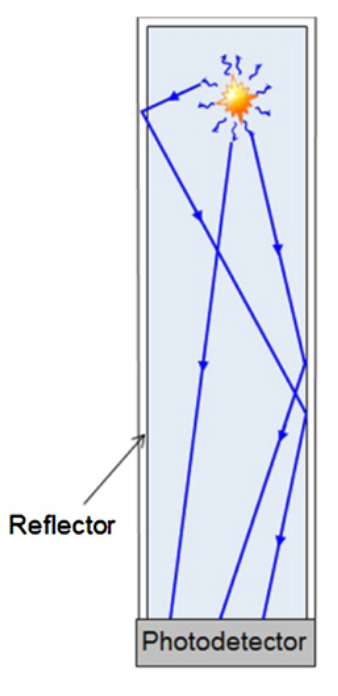
\includegraphics[scale=0.5]{images/scintillation.png}
  \scriptsize Reflection of optical photons within a scintillator. Image obtained from \cite{roncali_cherry_2013}.
  % \end{figure}
  \end{center}
  \end{column}
  \end{columns}

\end{frame}

\begin{frame}
\frametitle{GEANT4 Surface Treatment Models  }
\scriptsize 
\begin{itemize}
\item glisur (GEANT3) \\
Users indicate the value of polish, where a random point is generated in a sphere of radius (1-polished), and the corresponding vector is added to the average surface nominal normal as the micro-facet normal. A specular reflection is thereafter calculated based on the microfacet orientation. \cite{geant4_doc} \cite{janecek_moses_2010} \\
\ \\

\item unified \\
 Users specify a parameter $SigmaAlpha$, which defines the standard deviation of the Gaussian distribution of micro-facets around the average surface normal. \cite{geant4_doc} Four kinds of surface reflections are possible: specular, spike, lobe, backscatter and Lambertian. \cite{janecek_moses_2010} \\
 \ \\

 Note: Geant4 assumes that the four reflection type probabilities are constants, and not functions of incidence angles, which does not fully agree with measured data in Ref. \cite{janecek_moses_2010} \\
 \ \\

 % The probability of micro-facet normals populates the annulus of solid angle $sin(\alpha) d\alpha$ will be proportional to a gaussian of $SigmaAlpha$
\item LUT \\
Model is based on measured surface data with rough and polished finishes that can be coupled without reflectors, or in combination with a specular reflector (e.g. ESR) or a Lambertian reflector (e.g. Teflon). Coupling method can be air or optical grease. \cite{geant4_doc}
\end{itemize}
\end{frame}

\begin{frame}
\frametitle{Types of Reflection}


\begin{columns}
\begin{column}{0.4\textwidth}
\scriptsize
Surface reflections components: \\
\centering
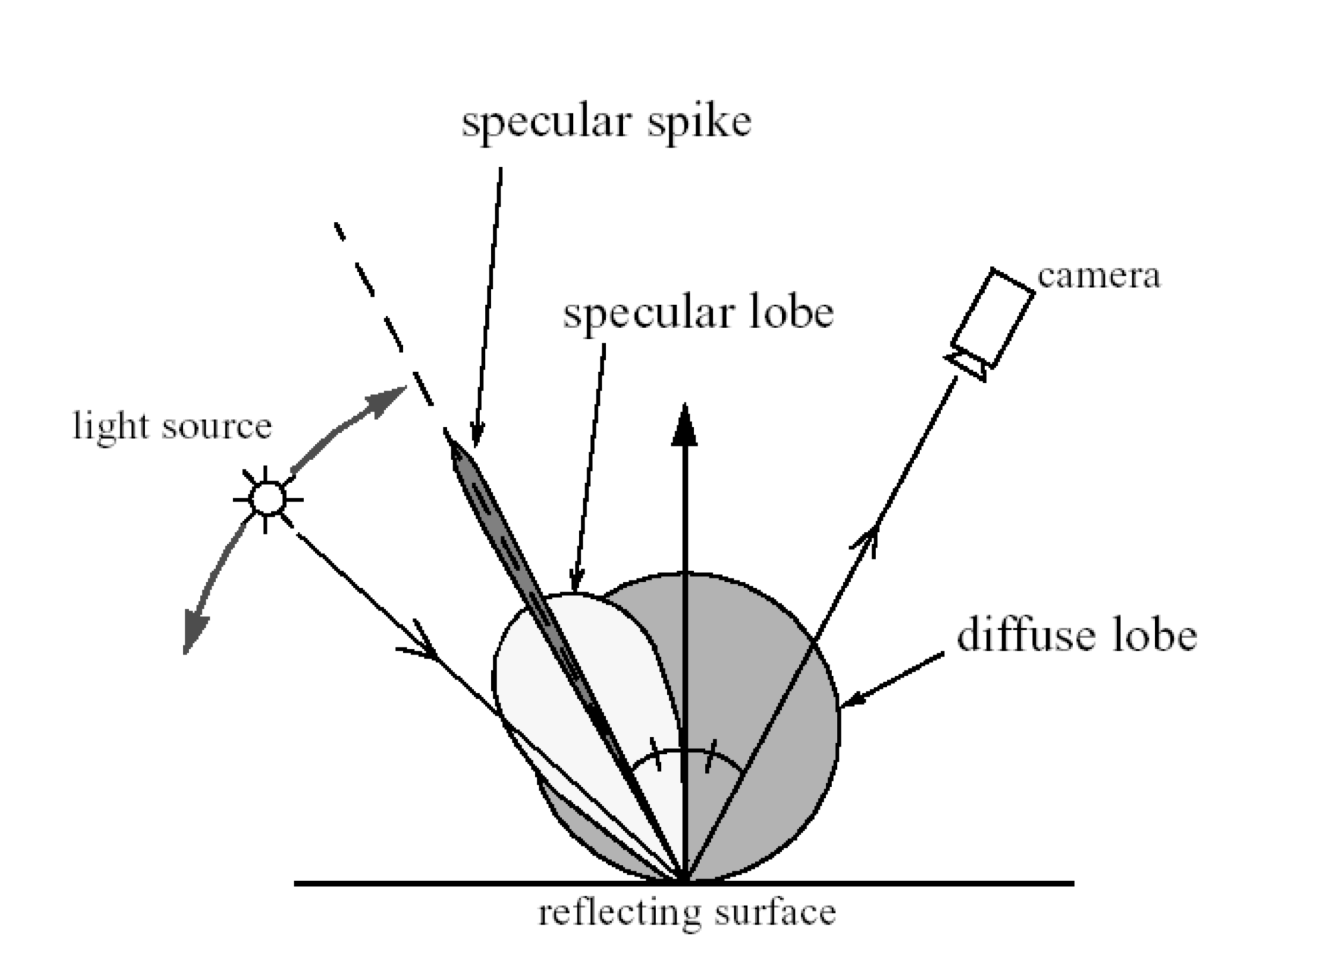
\includegraphics[width=\textwidth]{images/surface_reflection.png}
% \scriptsize
% \begin{block}{Note}
% % Unified model requires users to sepecify 4 reflection probability distributions, namely specular lobe, specular spike, backscatter and reflectivity.  
% Specular spike: the reflected photon is reflected about the average surface normal \\
% Backscatter: the photon is reflected by into the direction the photon came from \\
% Lambertian: the photon will be reflected with a Lambertian distribution (cosine distribution) about the average surface normal \\
% Specular lobe: the surface is assumed to consist of micro-facets, which are oriented around the average surface with a Gaussian distribution defined by $SigmaAlpha$. A micro-facet is randomly selected from the distribution defined by $SigmaAlpha$, and a specular reflection is thereafter calculated based on the micro-facet orientation. 
% \end{block}

\end{column}
\begin{column}{0.6\textwidth}
\scriptsize
\begin{block}{Terminology \cite{janecek_moses_2010}}
% Unified model requires users to sepecify 4 reflection probability distributions, namely specular lobe, specular spike, backscatter and reflectivity.  
\begin{tabular}{c p{4.5cm}}
Specular spike & the reflected photon is reflected about the average surface normal \\
Backscatter & the photon is reflected by into the direction the photon came from \\
Lambertian & the photon will be reflected with a Lambertian distribution (cosine distribution) about the average surface normal \\
Specular lobe & the surface is assumed to consist of micro-facets, which are oriented around the average surface with a Gaussian distribution defined by $SigmaAlpha$. A micro-facet is randomly selected from the distribution defined by $SigmaAlpha$, and a specular reflection is thereafter calculated based on the micro-facet orientation. 
\end{tabular}
\end{block}
% Specular
% 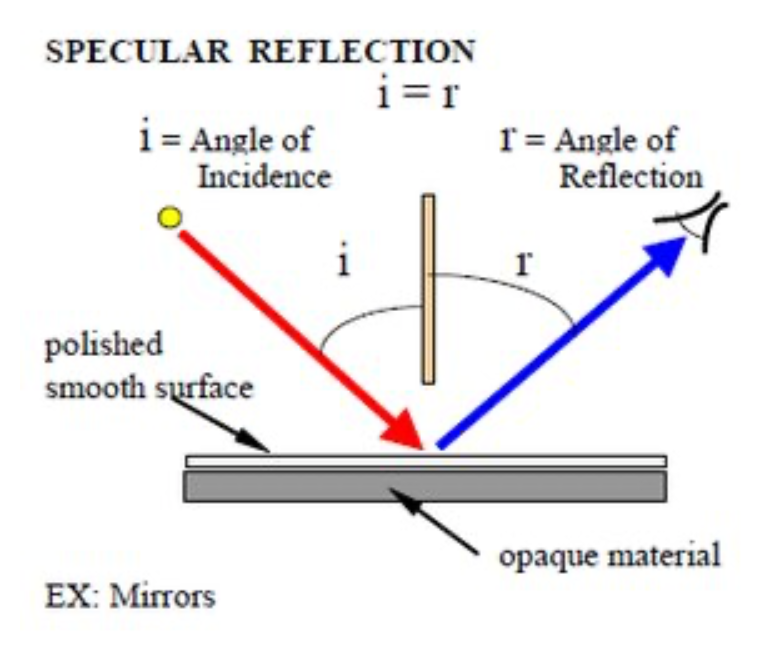
\includegraphics[width=0.8\textwidth]{images/specular.png}
% Lambertian
% 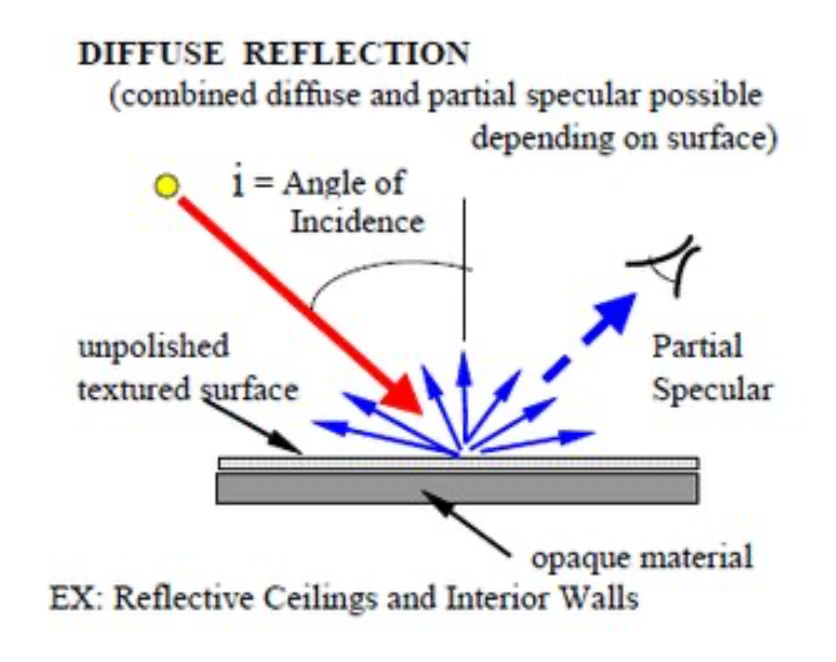
\includegraphics[width=0.8\textwidth]{images/lambertian.png}
\end{column}
\end{columns}
\end{frame}

\begin{frame}
\frametitle{Micro-Facets}
\centering
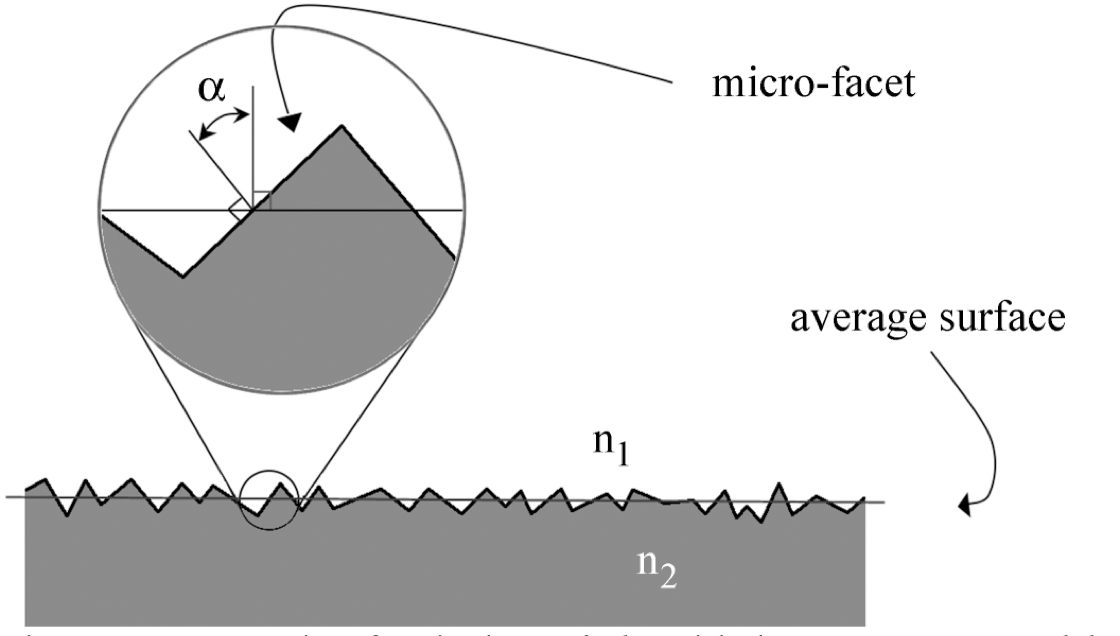
\includegraphics[width=0.6\textwidth]{images/microfacets.png}
\scriptsize \\
For a ground surface in the unified model, the parameter $SigmaAlpha$ defines the standard deviation of the Gaussian distribution of micro-facets around the average surface normal. \\ Image obtained from \cite{janecek_moses_2010}.

\begin{block}{Note}
Optical Monte Carlo software such as DETECT, Litrani, Geant4 or GATE allow the operator to set the surface reflections as purely specular, purely diffuse (Lambertian), or a linear combination of specular and Lambertian, which might not be a true representation of the real world. \cite{janecek_moses_2008}\\
\hfill  - Janecek, 2008
\end{block}
\end{frame}


\section{\scshape Simulation Model}
\begin{frame}
\frametitle{GEANT4 Simulation Model}
\scriptsize
Goals:
\begin{itemize}
\item Compare light collection based on different surface treatments (surface roughness, reflector type, coupling method) 
% Light collection efficiency based on crystal geometry, surface finish, reflector type and coupling method.
\item Estimate light sharing of monolithic scintillators over pixelated photodetectors
\end{itemize}
\ \\
\ \\
Key Model Parameters:
\begin{itemize}
\item Source: 
  \begin{itemize}
    \scriptsize
  \item monoenergetic neutron beam at 25 meV (1.8 \AA) 
  \item optical photons at 3.19 eV (395 nm)
  \end{itemize}
\item Geometry: single pixel and pixel array (8 $\times$ 8 pixels)
\item Material: $^6$Li-enriched glass scintillator (GS20, Scintacor)
\item Physics lists:
  \begin{itemize}
    \scriptsize
  \item QGSP\_BERT\_HP \\ energy of primary particle < 5 GeV, detailed neutron transport (< 20 MeV) 
  \item G4OpticalPhysics \\ optical photon transportation
  \end{itemize}
\item Output: ROOT files
\item Data Analysis: Python (Use uproot to read ROOT files)
\end{itemize}
\end{frame}

\begin{frame}
\frametitle{Primary particles}
Utilize a built-in primary particle generator $\rightarrow$ G4GeneralParticleSource: \\
\begin{columns}
\begin{column}{0.55\textwidth}

\begin{itemize}
\item Offers many pre-defined options 
  \begin{itemize}
  \item particle type \\ (neutron, gamma, proton, etc.)
  \item position distribution \\(point, plane, beam, etc.)
  \item angular distribution \\(isotropic, cosine-law, etc.)
  \item energy distributions \\(mono-energetic, power-law etc.)
  % \item multiple sources (user defined relative intensity) 
  \end{itemize}
\item Can be used via C++ or command line (or macro) UI
\end{itemize} 
\end{column}
\begin{column}{0.45\textwidth}
\begin{block}{Example GPS setup using macro}
$/gps/energy ~~0.025 ~eV$
$/gps/particle ~~neutron$
$/gps/direction ~~0. ~~0. ~~1.$
$/gps/pos/type ~~Beam$
$/gps/pos/shape ~~Circle$
$/gps/pos/sigma_r  ~~4 ~mm$ 
$/gps/pos/centre ~~0. ~~0. ~~-10. ~cm$
\end{block}
\end{column}
\end{columns}
\end{frame}

\begin{frame}
\frametitle{Detector Geometry}
Two detector geometry configurations: \\
\
\begin{columns}
\begin{column}{0.49\textwidth}
\centering
single pixel \\
\ \\
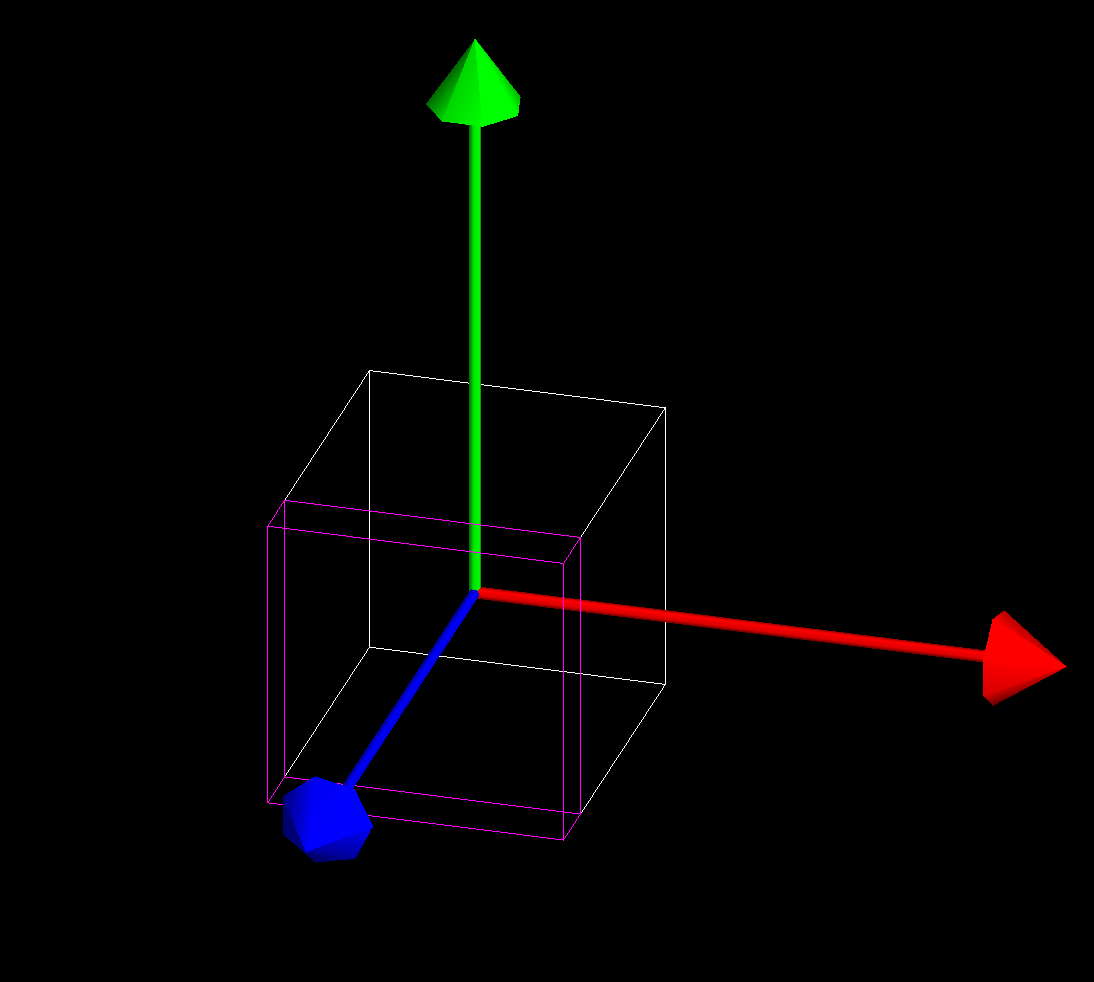
\includegraphics[width=\textwidth, height=5cm]{images/singlepixel.png}
\end{column}
\begin{column}{0.49\textwidth}
\centering
8 $\times$ 8 pixel array \\
\ \\
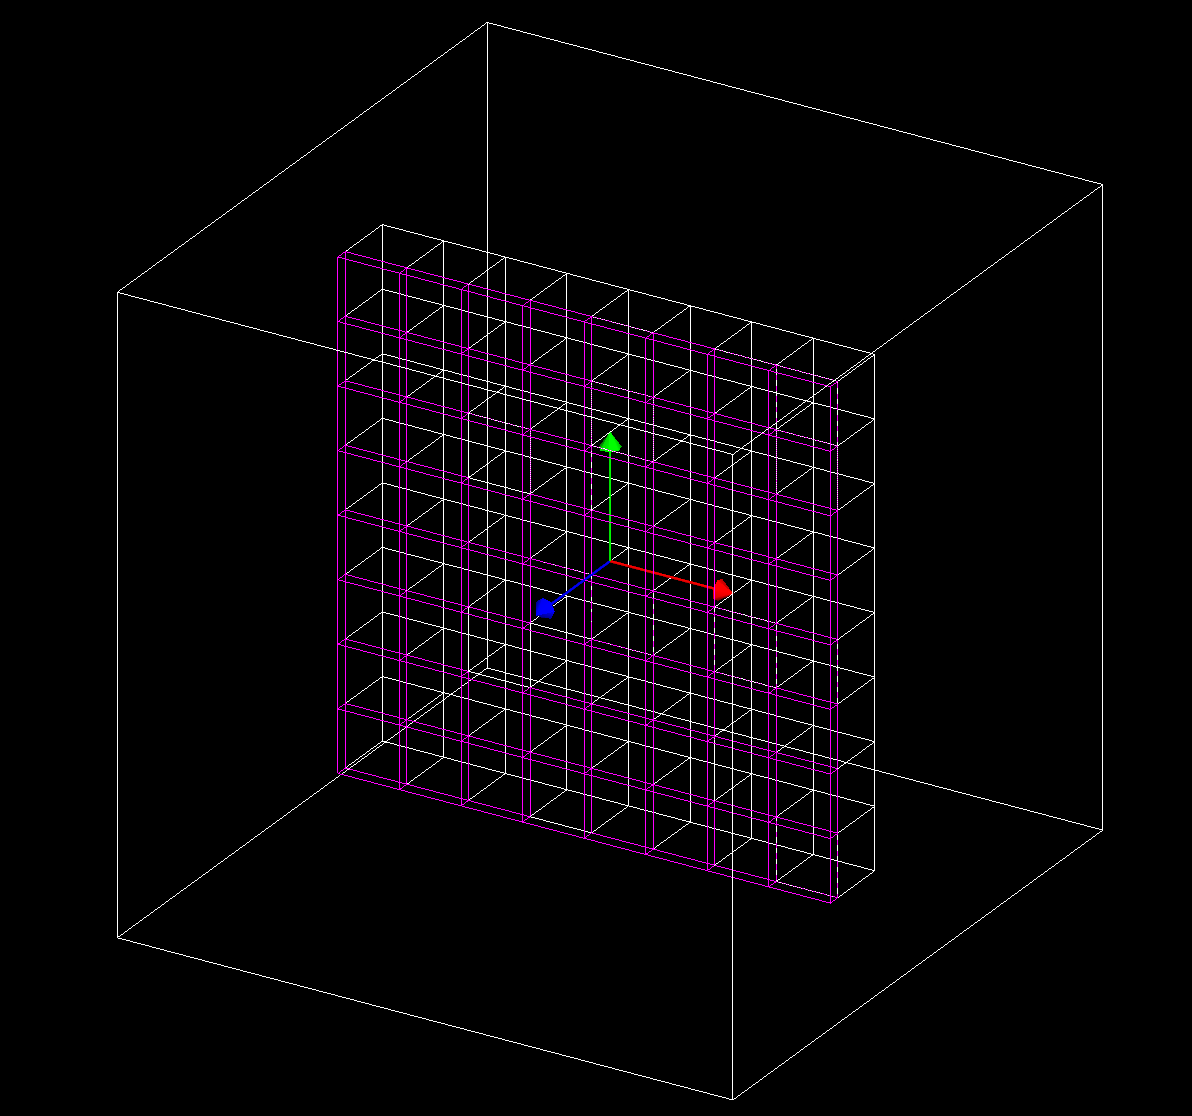
\includegraphics[width=\textwidth, height=5cm]{images/pixelarray.png}
\end{column}
\end{columns}
\ \\
\centering
scintillator (white wiring), photodetector (magenta wiring)
\end{frame}

\begin{frame}
\frametitle{Scintillator Material Composition and Properties}
\scriptsize
\begin{block}{Material Composition \cite{spowart_1976}}
\centering 
\begin{tabular}{p{1.7cm} | p{1.0cm} p{1.0cm} p{1.0cm} p{1.0cm} p{1.0cm} p{1.0cm} p{1.0cm}}
% \hline
 & SiO$_2$ & MgO & Al$_2$O$_3$ & Ce$_2$O$_3$ & Li$_2$O & Li & $^6$Li  \\
 \hline
Weight \% & 57 & 4 & 18 & 4 & 17.1 & 7.9 & 7.87 \\
% \hline
\end{tabular}
\end{block}
% \scriptsize \begin{center} Material composition of GS20 obtained from \cite{spowart_1976}. \end{center}

\begin{block}{Material Properties \cite{gs20}}
\centering \scriptsize
\begin{tabular}{c | c }
% \hline
Density (g/cm$^3$) & 2.50 \\
Wavelength$^\dagger$ (nm) & 395 \\
Refractive index$^\dagger$ & 1.55 \\
Decay time$^\ddagger$ (ns) & 18/57/98 \\
Scintillation yield$^{\dagger\dagger}$ (photons/MeV) &  \textasciitilde 1,276 \\
Linear attenuation coefficient$^{\ddagger\ddagger}$ (cm$^{-1}$) & 14.85 \\
Photon absorption length (cm) & 100 (assumed) \\
Yield ratio & 1.0 \\
Resoution scale & 1.0 \\
% \hline
\end{tabular}
\end{block}

\scriptsize  
$^\dagger$  at maximum emission. Full emission spectrum will be needed in simulation \\
$^\ddagger$ Fast component, slow component and 90\% to 10\% respectively \\
$^{\dagger\dagger}$ About 6,000 photons per absorbed neutron is normalized by the Q-value (4.73 MeV)\\
$^{\dagger\dagger}$ at thermal neutron energy (2meV) \\
% \begin{center}  Typical material properties of GS20 obtained from \cite{gs20}.  \end{center}

\end{frame}

\begin{frame}
\frametitle{Scintillator Boundary Interaction}
\scriptsize
% Parameters:
% \begin{itemize}
% \item Surface type 
% \item Optical surface mode 
% \item Optical surface finish 
% \end{itemize}

\begin{block}{Surface treatment}
\centering
\begin{tabular}{c | c }
% \hline
 surface type & dielectric-dielectric \\ %, dielectric-LUT $^\dagger$ \\
 % &  dielectric-LUTDAVIS $^\ddagger$\\
 model &  unified \\
 % , LUT, DAVIS   \\
 surface finish & rough, polished \\
 reflector type & air, TiO$_2$ \\ %teflon (lambertian), ESR (specular) \\
 % coupling method & air \\
 crystal thickness & 2 mm \\%1, 2, 6, 20 mm \\
 % \hline
\end{tabular}
\end{block}

% $^\dagger$ LUT model is based on BGO crystal. \cite{janecek_moses_2008} \\
% $^\ddagger$ DAVIS model is based on LYSO crystal \cite{roncali_cherry_2013} \\
% $^\dagger\dagger$ unified model

\begin{block}{Parameters for unified model \cite{janecek_moses_2010}}
\centering
\begin{tabular}{c | c}
$SigmaAlpha$  & 0.0227 rad/1.3$^o$ (polished) \\
& 0.209 rad / 12$^o$ (rough) \\
$REFLECTIVITY$ $^{\dagger}$ & 0.05 (air) \\
& 0.89 (TiO$_2$) \\
$RINDEX$ $^{\dagger}$ & 1.0 (air) \\
& 1.35 (TiO$_2$) \\
Reflection Type Probability $^{\dagger}$ & 100\% Diffuse lobe, 0\% specular lobe \\
& 0\% specular spike, 0\% backscatter \\
\end{tabular}
\end{block}
\centering 
\scriptsize $^{\dagger}$ Assume constant over all optical photon energies
\end{frame}




\section{\scshape Results and Discussions}

\begin{frame}
\frametitle{Detector Setup: Light Collection}
\scriptsize 
A single pixel is used to study the light collection with different surface treatments and scintillator thicknesses. Figure below shows a 2 mm x 2 mm x 2 mm scintillator cube with polished surfaces coupled to a layer of reflective coating. \\ 
\ \\
A neutron is emitted a distance away from the scintillator. Neutron is captured in the scintillator and approximately 6,000 photons are emitted isotropically. \\
\ \\
\centering
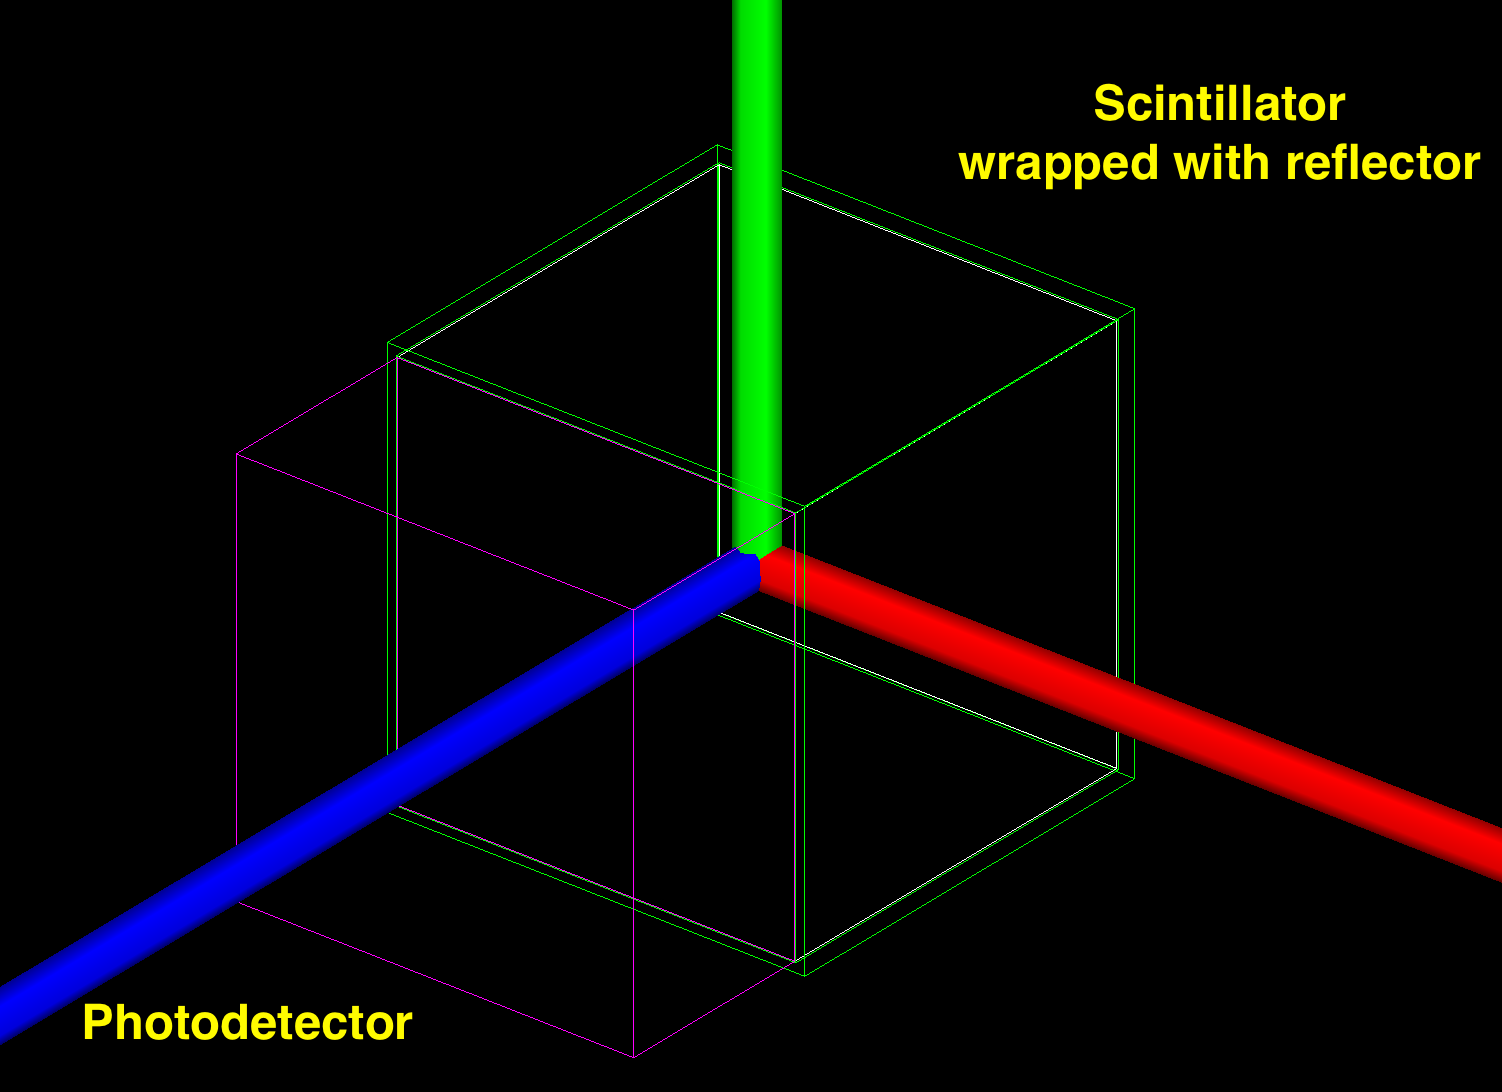
\includegraphics[width=0.48\textwidth, height=0.5\textheight]{images/scint_refl1.png}
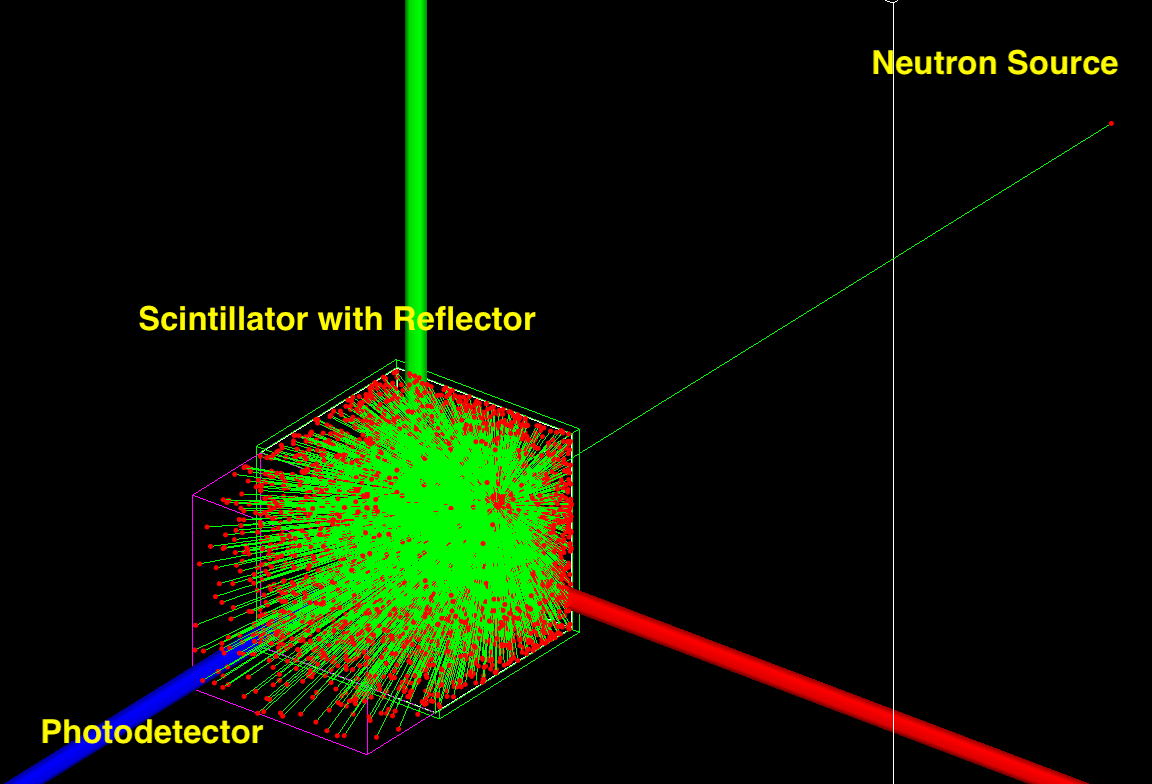
\includegraphics[width=0.48\textwidth, height=0.5\textheight]{images/scint_refl_neutron.png}
\end{frame}

\begin{frame}
  \frametitle{Validation: Neutron Capture}
  \scriptsize
  Here are an additional few plots that illustrate the expected results of neutron capture and energy deposited in the scintillator: \\
  \ \\
  \centering
  X-Y distribution: uniform distribution of neutron capture \\
  Z distribution: neutron attenuation of GS20 at 25 meV  \\
  Energy distribution: energy deposited by the reaction productions of neutron capture \\
   $^3$H (2.73 MeV) and $\alpha$ (2.05 MeV) \\
  \ \\
  
  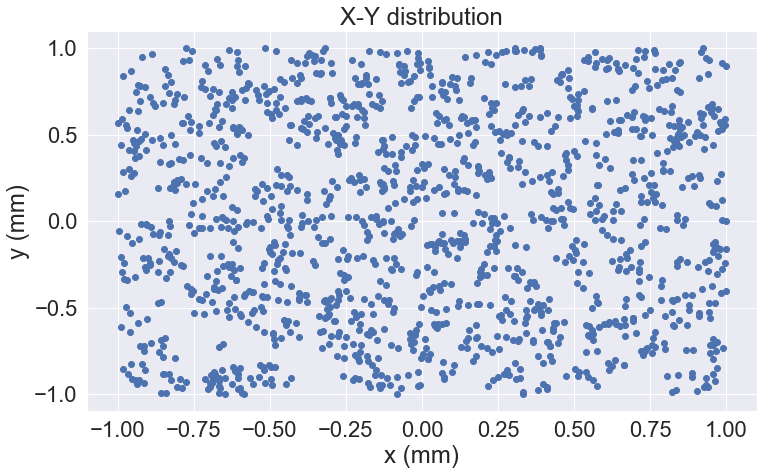
\includegraphics[width=0.32\textwidth, height=0.45\textheight]{images/xy_distribution1.png}
  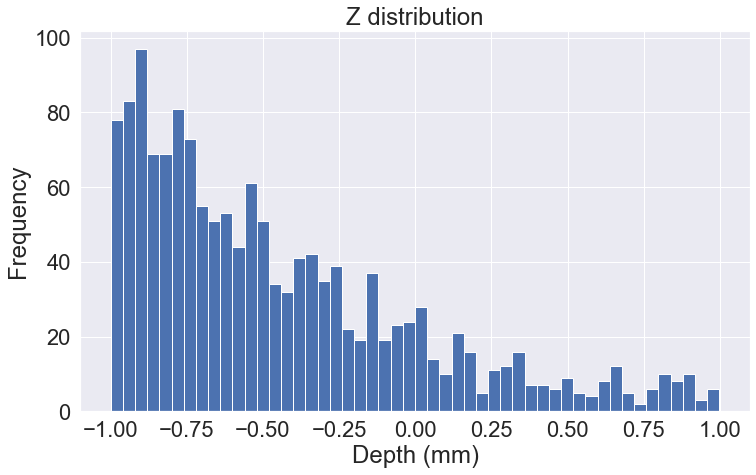
\includegraphics[width=0.32\textwidth, height=0.45\textheight]{images/z_distribution1.png}
  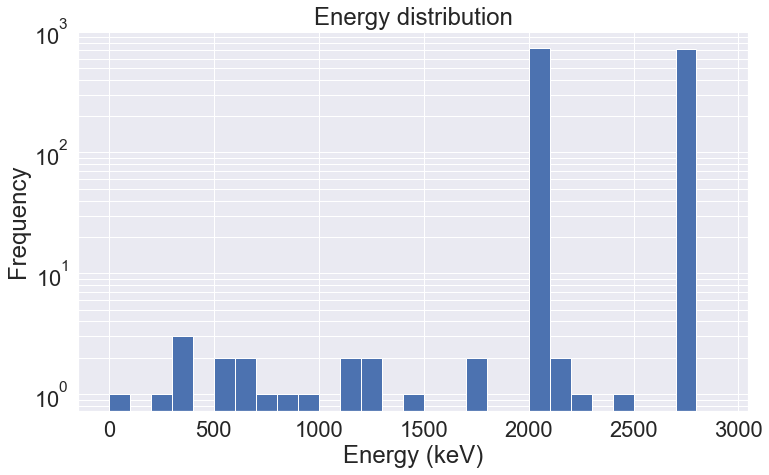
\includegraphics[width=0.32\textwidth, height=0.45\textheight]{images/energy_distribution1.png}
\end{frame}



\begin{frame}
  \frametitle{Validation: Optical Transport}
  \scriptsize 
  To make sure that the simulation of optical transport behaves as expected, 6,000 photons are emitted isotropically at 7 $\times$ 7 $\times$ 7 = 343 positions within the scintillator volume. Optical photons are used instead of neutrons to speed up simulation.\\
  \ \\
  Photodetector is positioned at z = 1.0 mm, where most photons are detected, as expected. The scintillator cube has a polished surface with no reflectors coupled to it.   \\
  \ \\
  \centering
  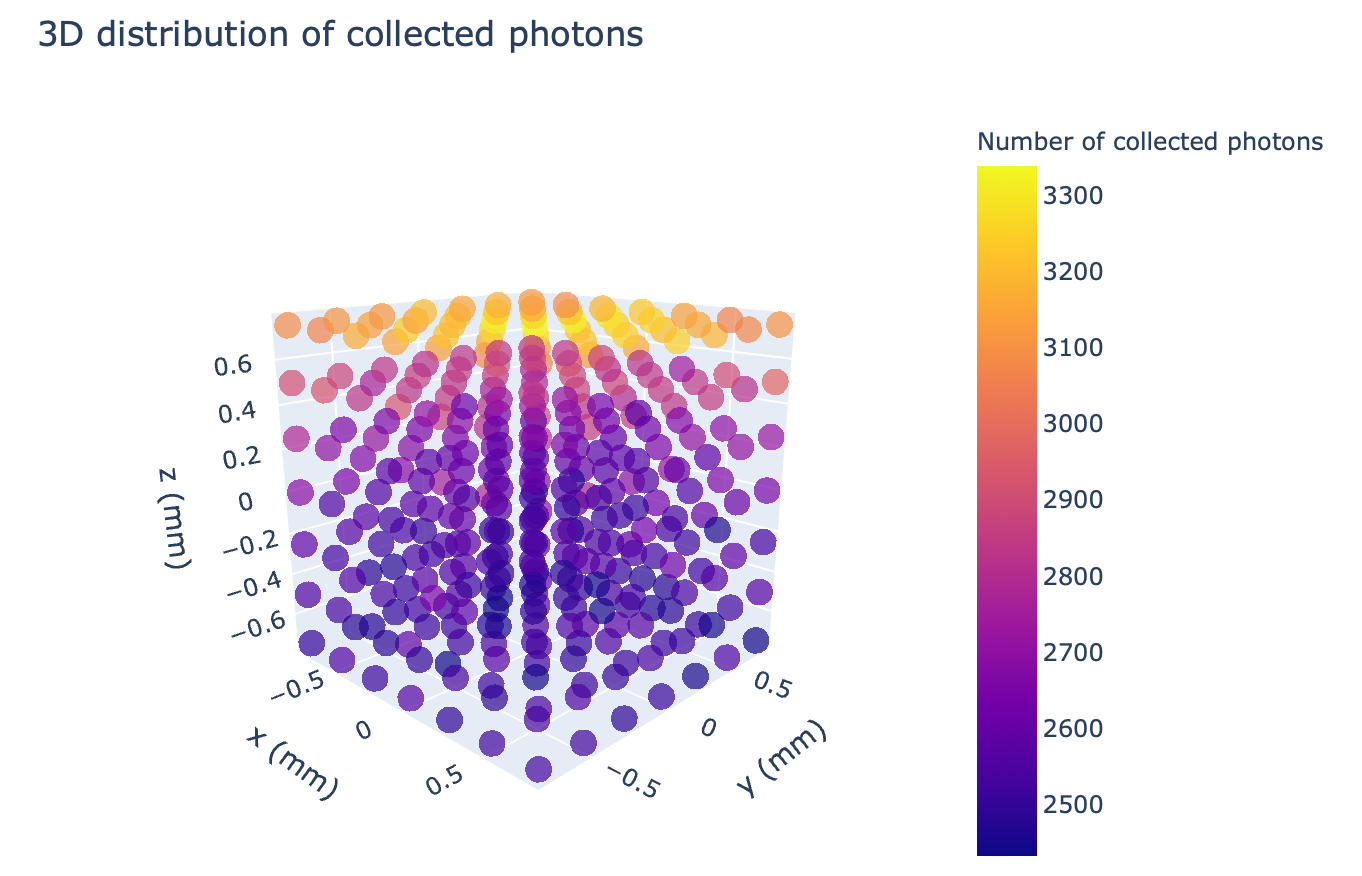
\includegraphics[width=0.49\textwidth, height=0.45\textheight]{images/distribution.png}
  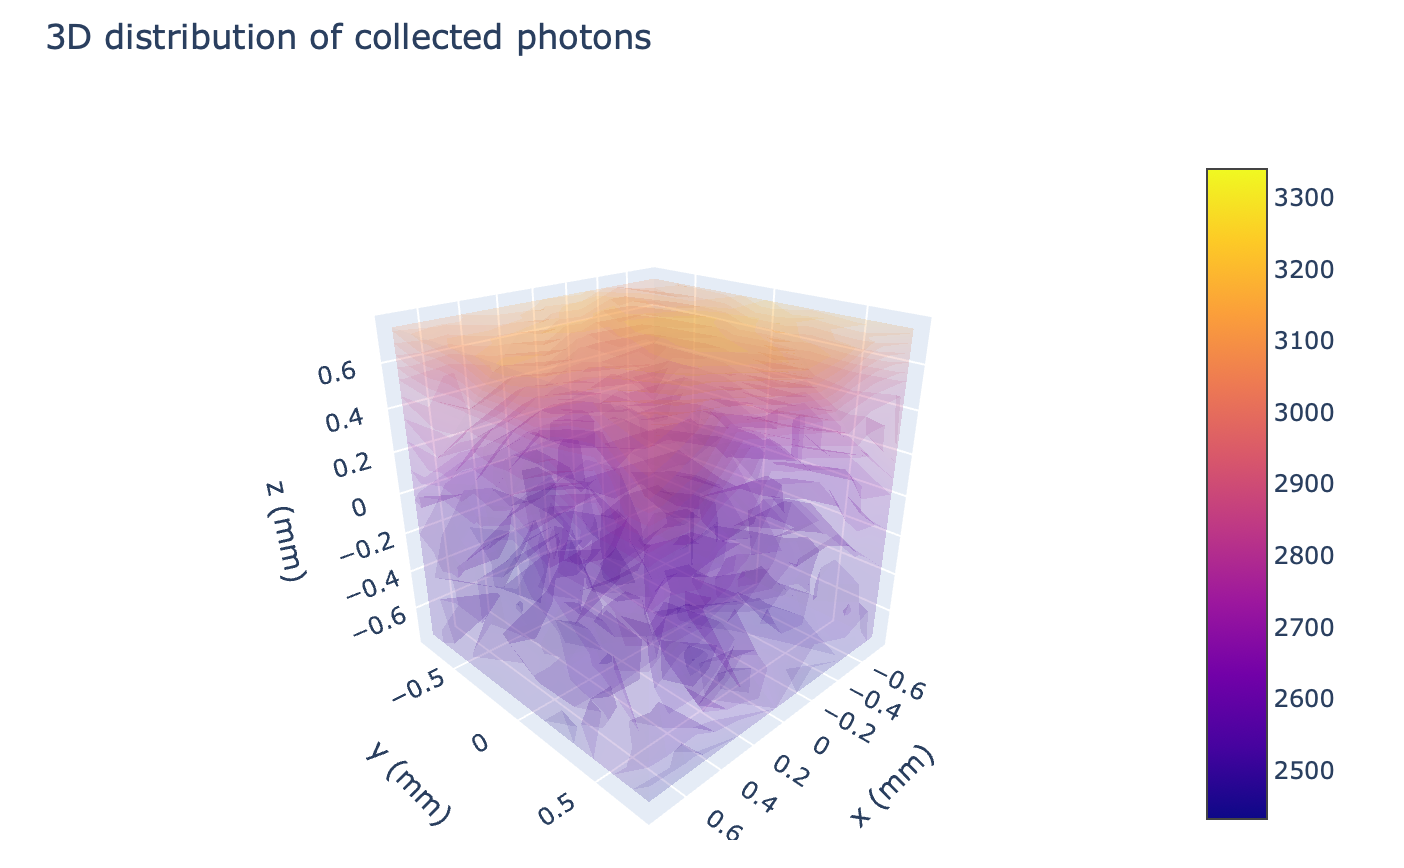
\includegraphics[width=0.49\textwidth, height=0.45\textheight]{images/distribution1.png}
  \ \\
\end{frame}

\begin{frame}
  \frametitle{Metric: Which is Better?}
  \scriptsize
  In Time-over-Threshold (ToT) spectrum, neutron peak with higher ToT values is better as it gives a better separation between neutron peak and gamma peak. \\
  \ \\
  Experimental data: \\
  % \ \\
  \centering 
  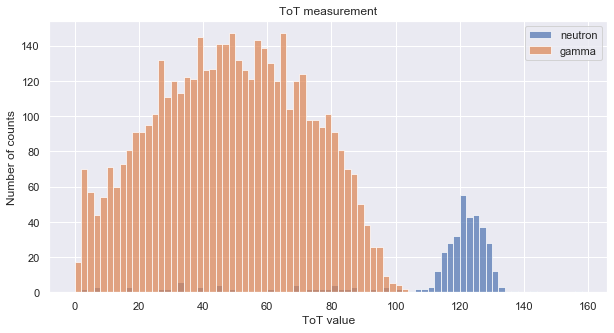
\includegraphics[width=0.49\textwidth, height=0.49\textheight]{images/roughness3.png}
  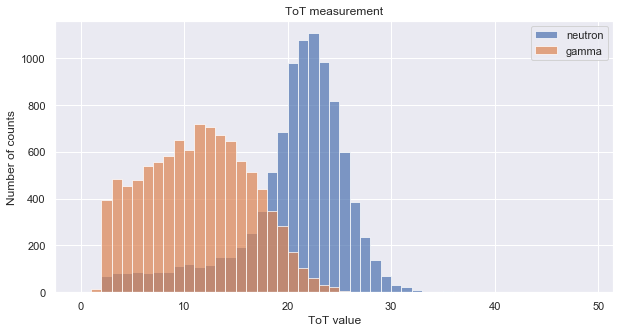
\includegraphics[width=0.49\textwidth, height=0.49\textheight]{images/spectra3.png}
  \flushleft~~~~~~~~~~~~~~~~~ 6 $\times$ 6 mm$^2$ SiPM \hspace{4cm} 1 $\times$ 1 mm$^2$ SiPM \\
  \ \\
  $^*$ The separation difference between neutron peak and gamma peak has to do with the active area of the SiPM. If the active area of SiPM is smaller than the area of the scintillator surface coupled to the SiPM (2 $\times$ 2 mm$^2$), less photons are collected as a results.  
\end{frame}

\begin{frame}
\frametitle{Results: Surface Treatments I}
\scriptsize
The simulation model is able to produce results that are consistent with experimental data when the scintillator surface is polished. \\
\ \\
Since the experimental data is not normalized, results can only be compared in relative. Both experimental and simulated results show that scintillator coupled with reflective coating have higher ToT values than the ones without. \\
\ \\
\centering 
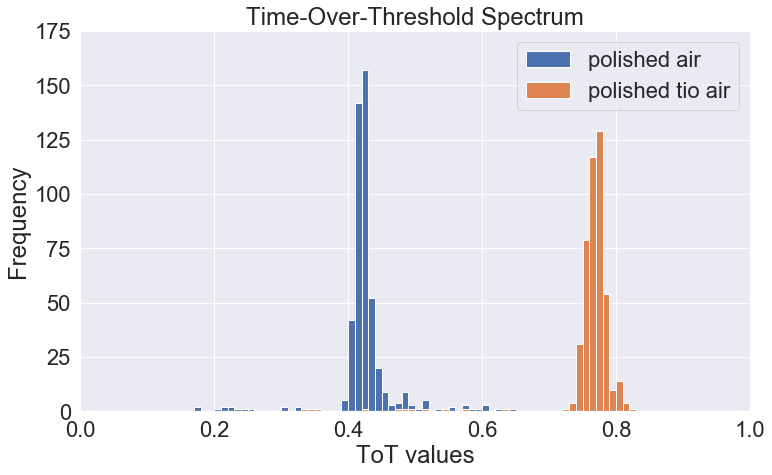
\includegraphics[width=0.49\textwidth, height=0.49\textheight]{images/comparison_polishedair_polishedtioair.png}
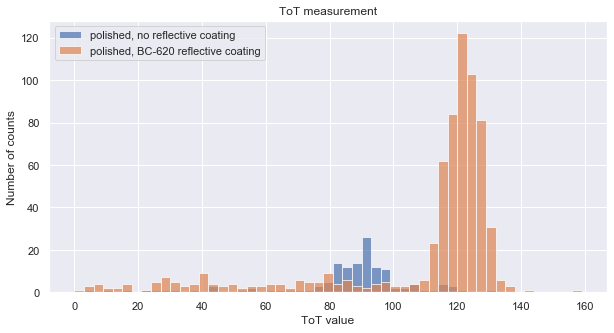
\includegraphics[width=0.49\textwidth, height=0.49\textheight]{images/roughness2.png}
\flushleft~~~~~~~~~~~~~~~~~~~~~ Simulated result \hspace{3cm} Experimental result
\end{frame}

\begin{frame}
\frametitle{Results: Surface Treatments II}
\scriptsize
The simulation model is not able to model rough surfaces well. This result is expected and published in numerous articles. \cite{janecek_moses_2008} \cite{janecek_moses_2010} \cite{roncali_cherry_2013} \cite{roncali_stockhoff_cherry_2017}  \\
\ \\
The next slide will show published result from \cite{janecek_moses_2010} that shows the discrepancy between simulated data and experimental data using Geant4 unified model. \\
\ \\
\centering
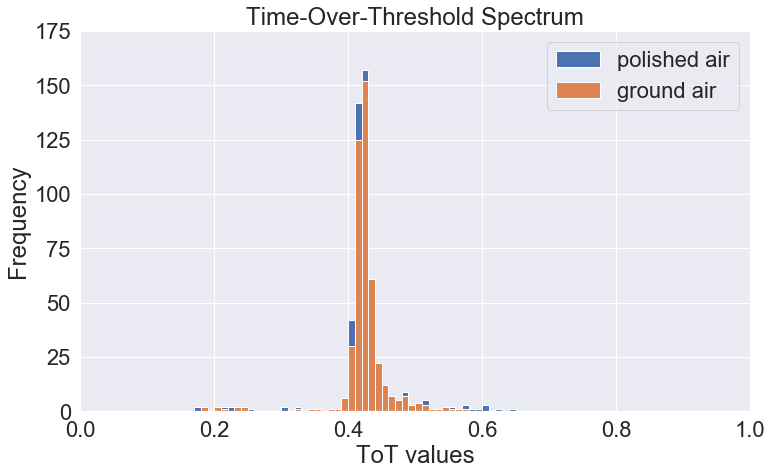
\includegraphics[width=0.49\textwidth, height=0.45\textheight]{images/comparison_groundair_polishedair.png}
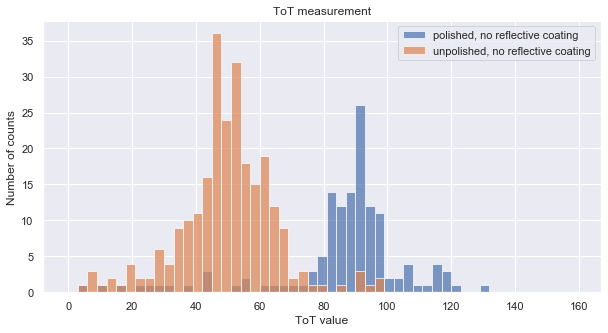
\includegraphics[width=0.49\textwidth, height=0.45\textheight]{images/roughness1.png}
\flushleft~~~~~~~~~~~~~~~~~~~~~ Simulated result \hspace{3cm} Experimental result
% 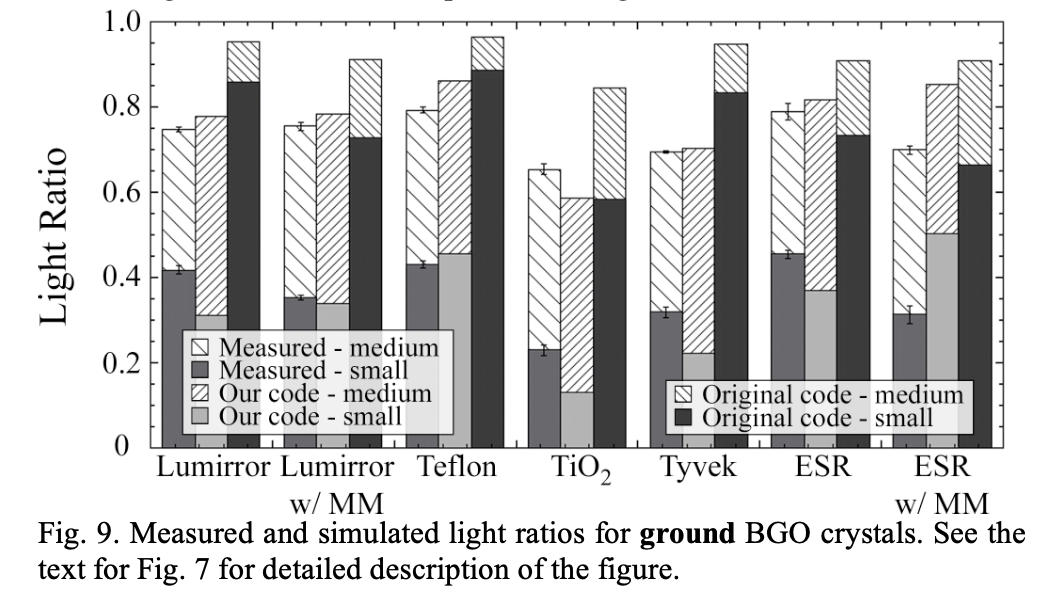
\includegraphics[width=0.49\textwidth, height=0.45\textheight]{images/bgo_rough.png}
% 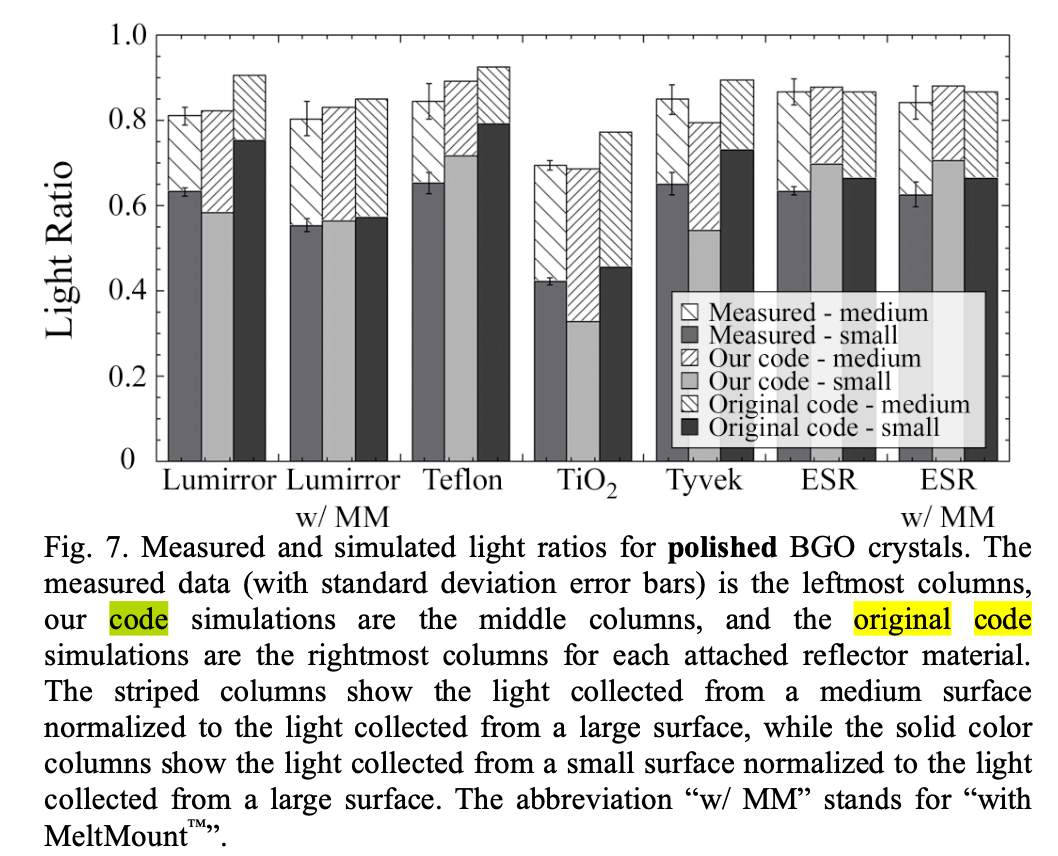
\includegraphics[width=0.49\textwidth, height=0.45\textheight]{images/bgo_polished.png}
\end{frame}

\begin{frame}
\frametitle{Results: Surface Treatments III}
\scriptsize
The original code (using Geant4 unified model) perform better in simulating polished surfaces than rough surfaces as the discrepancies between simulated data and measured data are smaller. \\
\ \\
Using Geant4 unified model, the simulated light yield tends to be higher for rough surfaces than for smooth surfaces. Meanwhile, measured data generally shows that the light yield for polished surfaces are higher than rough surfaces. 
\ \\
\centering
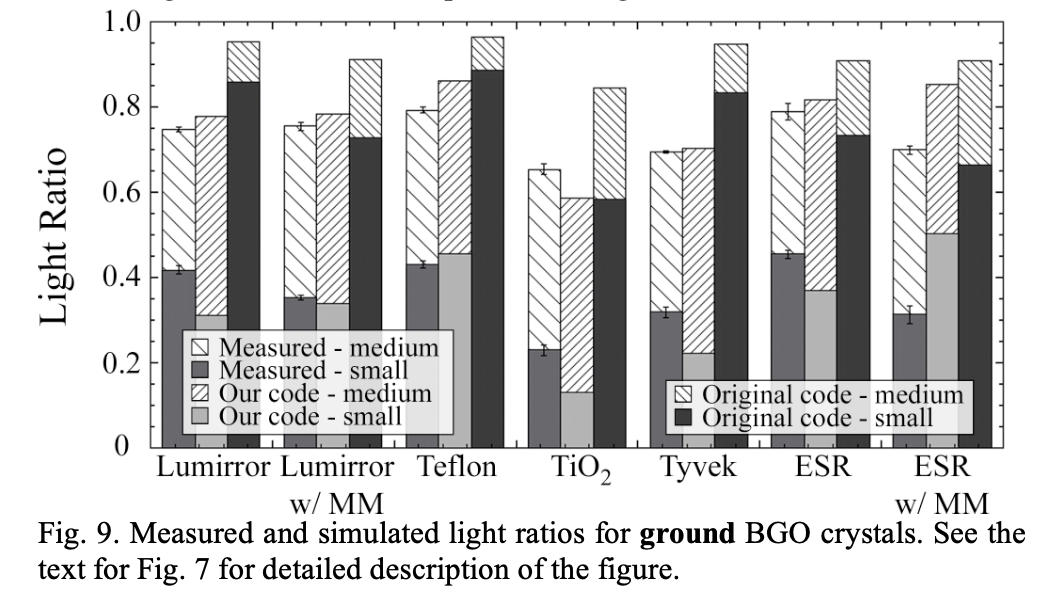
\includegraphics[width=0.49\textwidth, height=0.45\textheight]{images/bgo_rough.png}
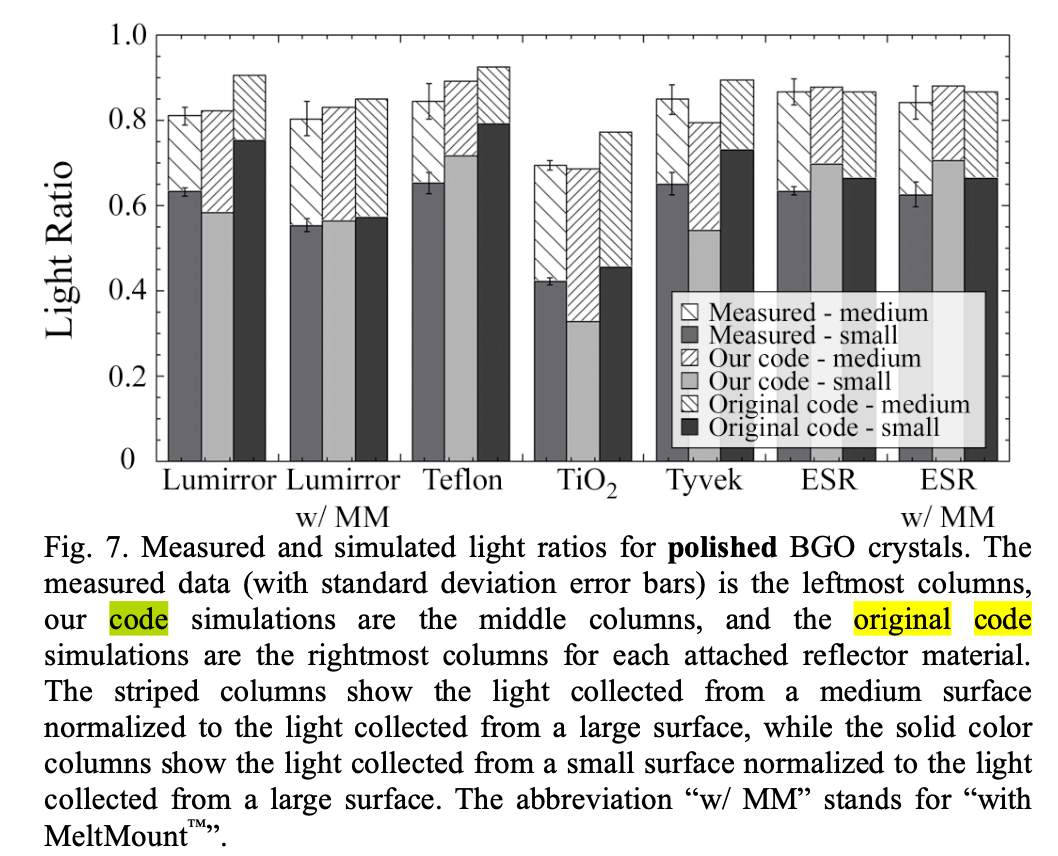
\includegraphics[width=0.49\textwidth, height=0.6\textheight]{images/bgo_polished.png}
\flushleft~~~~~~~~~~~~~~~~~~~~~ Rough \hspace{5cm} Polished
\end{frame}

\begin{frame}
  \frametitle{Results: Scintillator Thickness}
  \scriptsize
  The effect of aspect ratio on the light output of scintillator. It has been demonstrated that crystals shaped in thin rods have a lower light output as compared to bulky or sliced crystals. \cite{pauwels_2012} \\
  \ \\
  Since our simulation model works well with polished surfaces, we only investigated two polished surface treatments. The simulated result is consistent with the result published in \cite{pauwels_2012}. \\
  \ \\
  \centering
  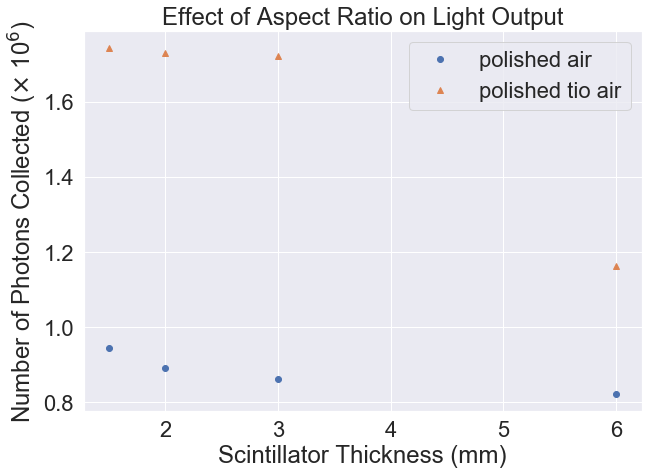
\includegraphics[width=0.49\textwidth, height=0.49\textheight]{images/light_yield_thicknesses.png} 
  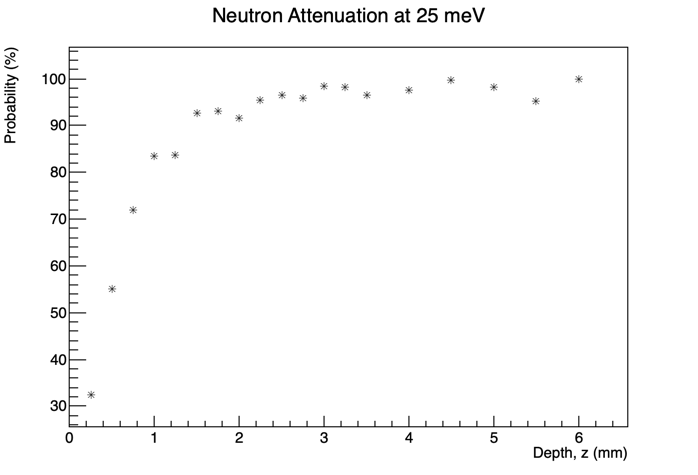
\includegraphics[width=0.49\textwidth, height=0.49\textheight]{images/gs20_attenuation_simulated.png}
  \flushleft Experimental validation is needed to find the optimum scintillator thickness for maximum light output.
\end{frame}

\begin{frame}
\frametitle{Simulated Detector Setup}
\scriptsize
Having pixelated scintillator arrays often requires cutting, polishing, applying reflective coating and optical grease and assembling scintillator arrays to couple to SiPM, hence results in higher cost and more laborious. \ \\
\ \\
We are interested to investigate the effect of monolithic scintillator thickness on the crosstalk/light sharing between pixels. \\
\ \\
\centering 
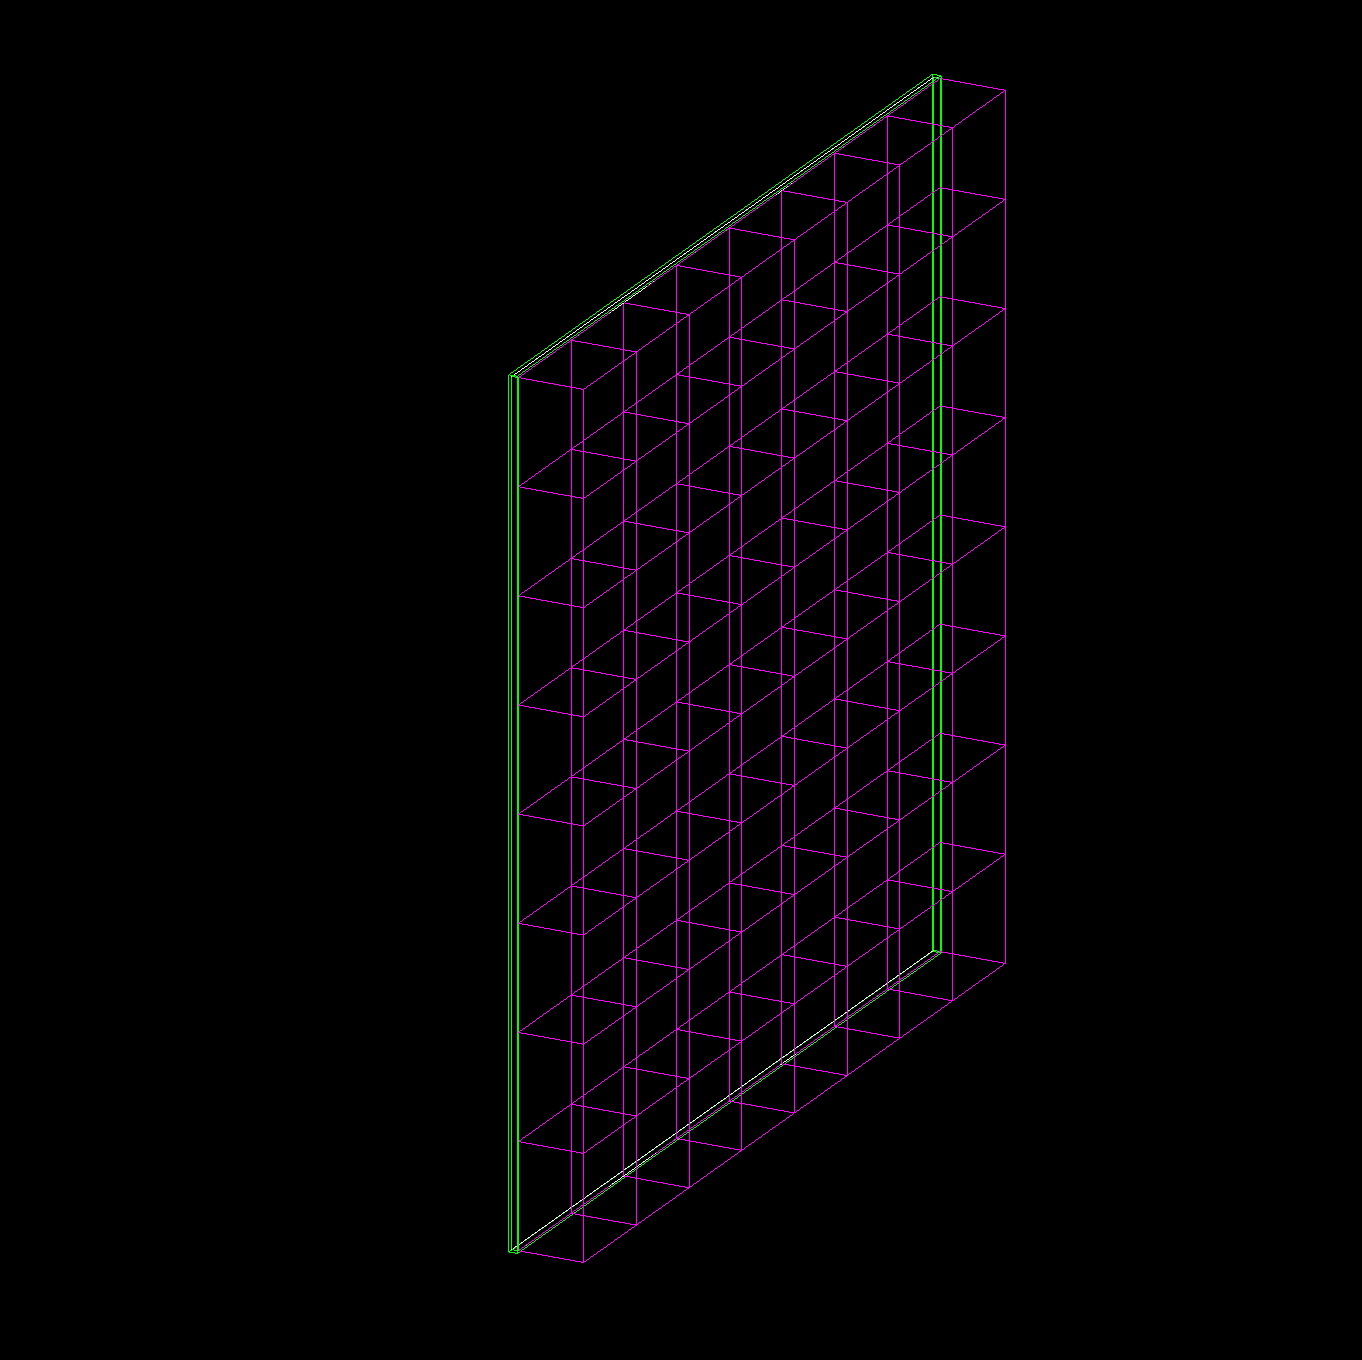
\includegraphics[width=0.48\textwidth, height=0.49\textheight]{images/monolithic_pixelarray.png}
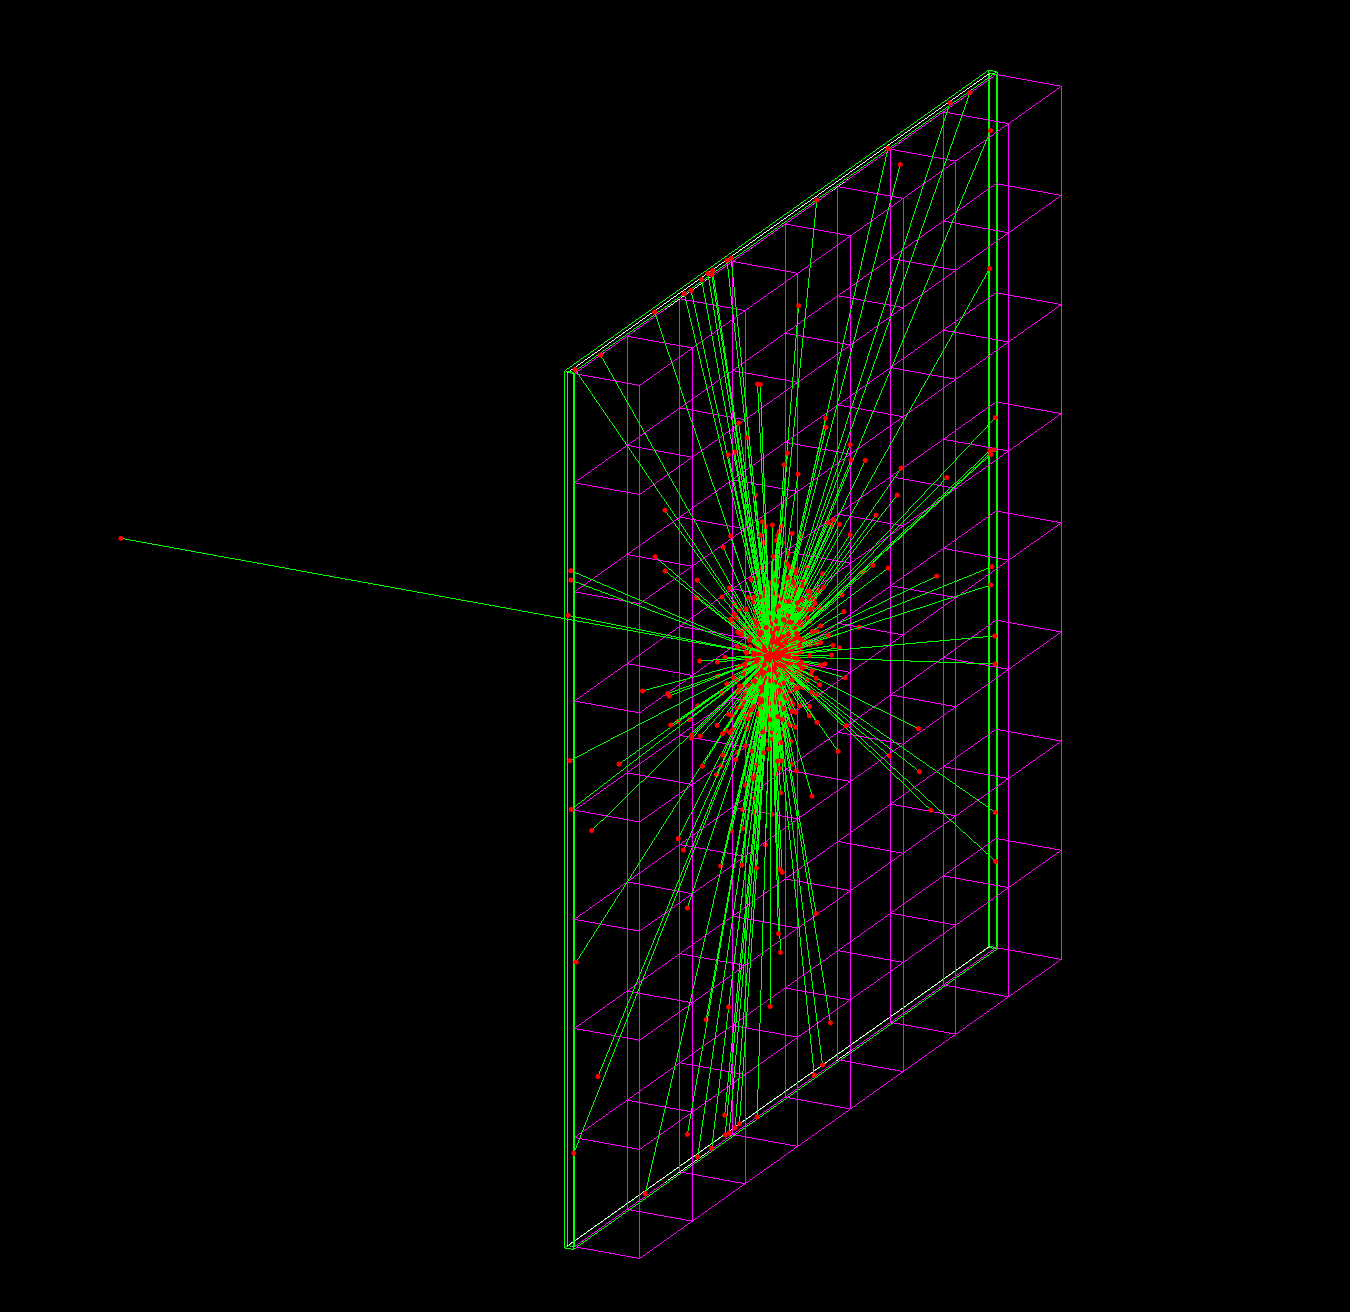
\includegraphics[width=0.48\textwidth, height=0.49\textheight]{images/monolithic_pixelarray1.png}
\end{frame}

\begin{frame}
\frametitle{Results: Light Sharing / Crosstalk }
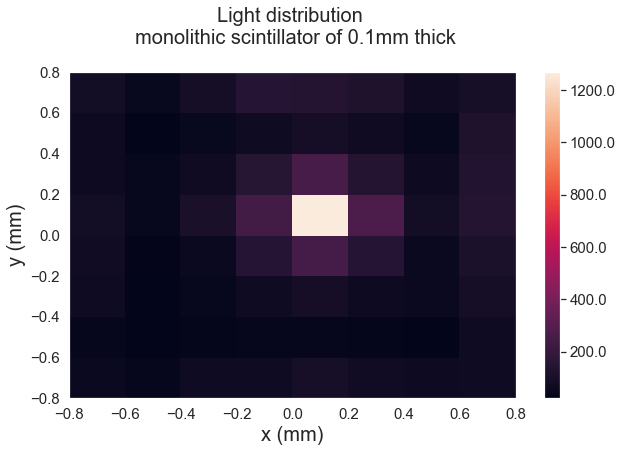
\includegraphics[width=0.49\textwidth, height=0.4\textheight]{images/hist2d_0p1mm.png}
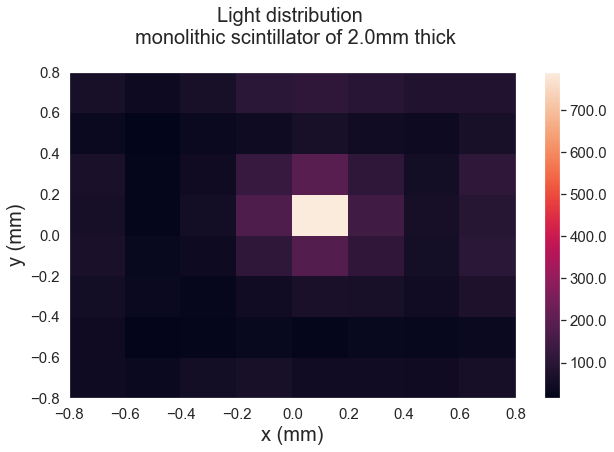
\includegraphics[width=0.49\textwidth, height=0.4\textheight]{images/hist2d_2mm.png}
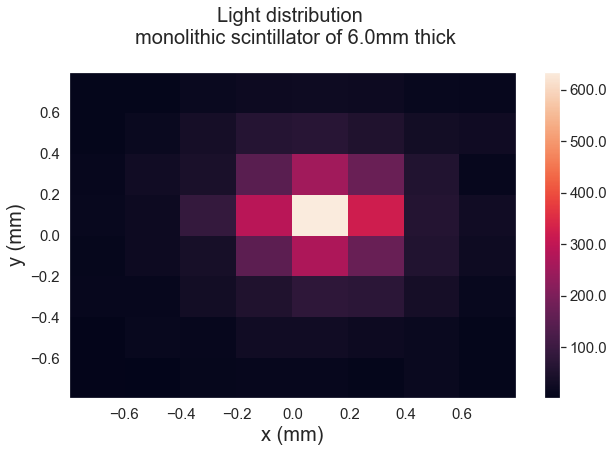
\includegraphics[width=0.49\textwidth, height=0.4\textheight]{images/hist2d_6mm.png}
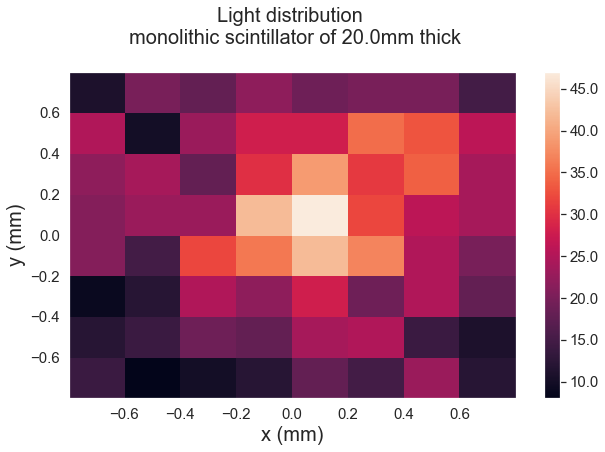
\includegraphics[width=0.49\textwidth, height=0.4\textheight]{images/hist2d_20mm.png}
\end{frame}

\begin{frame}
\frametitle{Light Sharing Between Pixels}
\scriptsize
Quantify cross talk using the percent difference in count rates between the first nearest neighbors and the second nearest neighbors.
\begin{columns}
\begin{column}{0.6\textwidth}
\begin{block}{Results}
\centering
\begin{tabular}{p{2cm} | c c}
Scintillator thickness (mm) & Crosstalk (\%) & Target (counts) \\
\hline
0.1 & 65.93 & 1268 \\
2.0 & 65.25 & 790 \\
6.0 & 75.42  & 634 \\
20.0 & 73.36 & 47 \\
\end{tabular}
\end{block}
\end{column}
\begin{column}{0.35\textwidth}
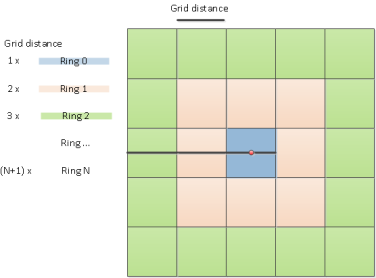
\includegraphics[width=0.9\textwidth]{images/knn.png}
\end{column}
\end{columns}

\begin{block}{Discussion}
\begin{itemize}
\item The overall crosstalk using monolithic scintillator is still much larger than segmented scintillator (experimentally measured to be about 5.64\%)
\item Monolithic scintillator results in the whole detector area to be dead during scintillations $\rightarrow$ lower detection rate
\end{itemize}
\end{block}
\end{frame}

\section{\scshape Conclusion and Future Work}
\begin{frame}
\frametitle{Conclusion}
\scriptsize
\begin{itemize}
\item Geant4 unified model can model polished surfaces relatively well, but performs rather poorly on rough surfaces. This may be due to the model description on surface roughness is not a true representation of the actual surfaces. 
\item The aspect ratio of the scintillator affects the light output. Crystal shaped in thin rods have a  lower light output as compared to bulky or sliced crystals. 
\item Monolithic scintillator in a pixel array configuration results in much larger cross talk between photodetector pixels than pixelated scintillator, even with scintillator thickness of 100 $\mu$m.
\end{itemize}

\begin{block}{Key results}
\begin{itemize}
  \item Coupling of reflective coating helps with light collection for polished surfaces, evidenced by both experimental and simulated results.
  \item Segmentation in scintillator is necessary to prevent crosstalk/light sharing between pixels and increase the counting rate of the detector. 
\end{itemize}
\end{block}
% Challenges in optical simulation using GEANT4:
% \begin{itemize}
% \item A simplified description of rough surfaces as an ensemble of micro-facets determined by the distrubution of Gaussian distribution may not be the true representation of surface roughness.
% \item Optical reflectance of a material may not be a linear combination of backscatter spike, specular spike, specular lobe and Lambertian reflections. 
% \item Two published results demonstrated the discrepancies between GEANT4 unified models and experimental data and obtained better accuracy by using measured reflectance data in simulation modelling without making assumptions about the surface roughness.
% \end{itemize}
\vfill
\end{frame}

\begin{frame}
\frametitle{Future Work}
\scriptsize
\begin{itemize}
  \item Lack of experimental data \\
    \begin{itemize}
      \scriptsize
      \item Light output of different scintillator thicknesses to find the optimal scintillator thickness for maximum light collection
      \item Effect of monolithic scintillator thickness on crosstalk/light sharing between pixels to validate that pixelation in scintillator is necessary for minimal crosstalk and high counting rate
     
    \end{itemize}

  \item Interest of time \\
  \begin{itemize}
    \scriptsize
    \item The reflectance and transmitance of light on the scintillator with different surface treatments can be measured and incorporated in the look up table (LUT) model in Geant4. 
    \item Better results has been shown in modelling rough surfaces. 
    \item Future optical transport simulation on GS20 can be available to public. 
  \end{itemize}
\end{itemize}

\vfill
\end{frame}

% \begin{frame}
% \frametitle{Acknowledgement}
% Most of the framework can be obtained from Dr. Micah Folsom's public Github repository. (https://github.com/micahfolsom/mgg4)
% \end{frame}

\frame[noframenumbering, plain]{\frametitle{References}
\tiny{\bibliographystyle{plain}}
\bibliography{bib/bib}
}

\appendix

\section{Backup Slides}
% \begin{frame}[noframenumbering, plain]
% \frametitle{Equations}
% Snell's law:
% $$ n_i ~sin(\theta_i) = n_t ~sin(\theta_t) $$

% Critical angle:
% $$ \theta_c = sin^{-1}(n_t/n_i) $$
% \end{frame}

\begin{frame}[noframenumbering, plain]
\frametitle{Relevant Published Data}
\begin{block}{Scintillator crystal without any reflectors: }
\centering \scriptsize
\begin{tabular}{ c | c c c}
& GS20 & LYSO & BGO \\
\hline
Refractive Index & 1.55 & 1.81 & 2.15 \\
Critical angle ($^o$) & 40.18 & 33.53 & 26.23 \\ 
Wavelength at maximum emission (nm) & 395 & 420 & 480 \\
\end{tabular}
\end{block}

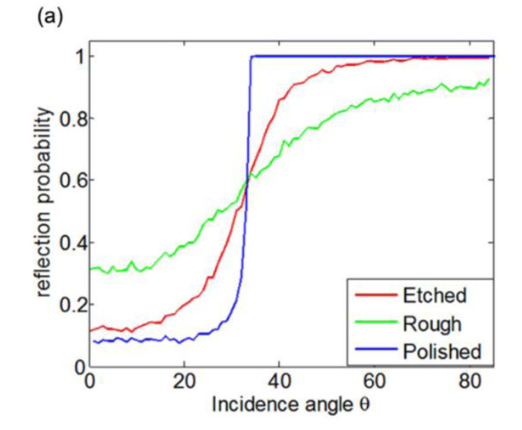
\includegraphics[width=0.49\textwidth, height=0.45\textheight]{images/LYSO_reflectivity_angular_distribution.png}
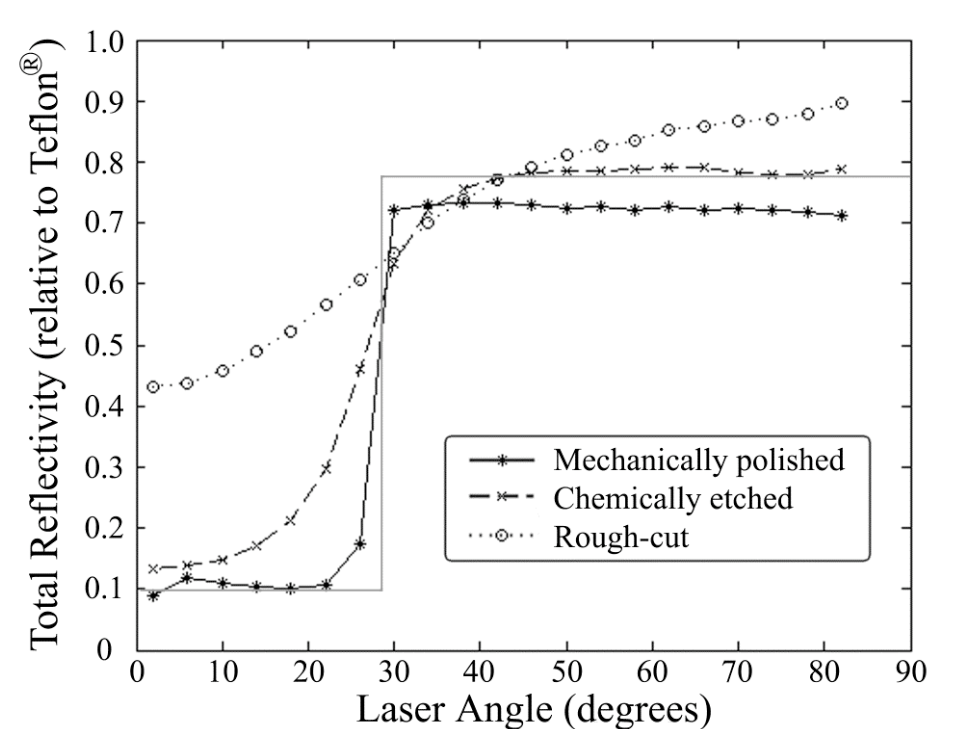
\includegraphics[width=0.49\textwidth, height=0.45\textheight]{images/BGO_reflectivity_angular_distribution.png}
\scriptsize \flushleft~~~~~~~~~~~~~~~~~~~~~~~~ LYSO \cite{roncali_stockhoff_cherry_2017} \hspace{5cm} BGO \cite{janecek_moses_2010} \hspace{3cm}
\end{frame}

\begin{frame}[noframenumbering, plain]
\frametitle{Relevant Published Data}
Several reflectors exhibits "cut-offs" for the reflectivity for shorter wavelengths, such as TiO$_2$ (420 nm) and ESR film (395 nm). \cite{janecek_2012} \\
\ \\
Reflectivity curve as a function of wavelengths: \\
\ \\
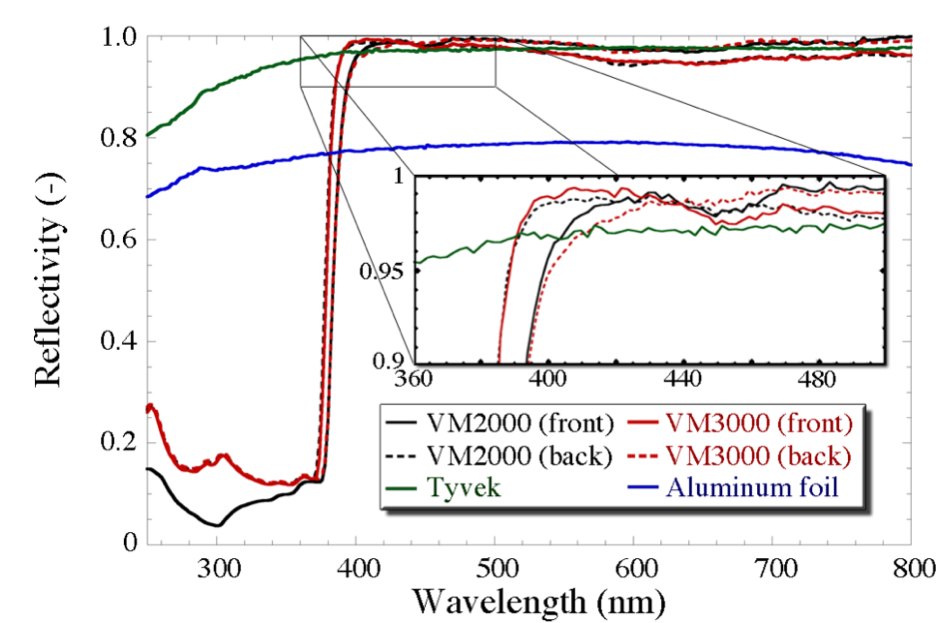
\includegraphics[width=0.49\textwidth, height=0.45\textheight]{images/vm2000_reflectivity_curve1}
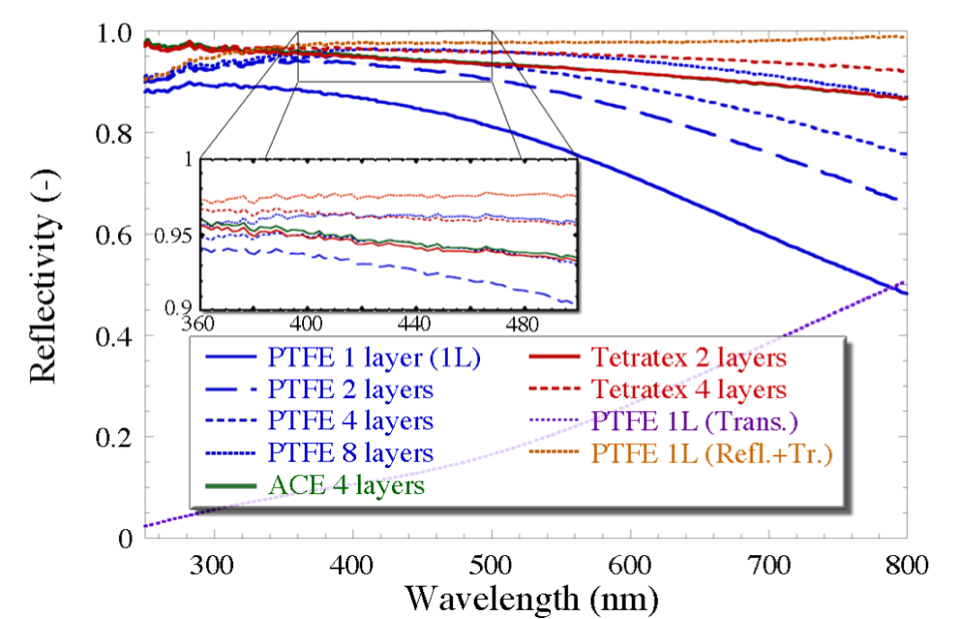
\includegraphics[width=0.49\textwidth, height=0.45\textheight]{images/teflon_reflectivity_curve1}
\scriptsize \flushleft~~~~~~~~~~~~~~~~~~~~~~~ VM2000 \cite{janecek_2012}  \hspace{5cm} Teflon \cite{janecek_2012} \hspace{3cm}
\end{frame}

% \begin{frame}[noframenumbering, plain]
%   \vspace{3cm}
%   \centering
%   Thank you for your time!
%   \vspace{3cm}
% \end{frame}

\end{document}